% Introduction to Newton's Method
% Source: https://stats.stackexchange.com/questions/376191/why-is-the-second-derivative-required-for-newtons-method-for-back-propagation
% Source: https://tutorial.math.lamar.edu/classes/calci/newtonsmethod.aspx
% Spring 2021



\qns{Newton's Method Introduction}

\meta{In this problem, we will review Newton's method, which was introduced in lecture.}

The newton's method that you may have heard of in calculus class is typically used for finding the roots of a function.
Recall that the roots of a function are the inputs such that the output is zero.

For example, suppose that we have the function $f(x) = x^{2} + 5x + 6$.
Factorizing into $f(x) = (x+2)(x+3)$ reveals that the roots of this function are $x=-2, -3$.

\begin{center}
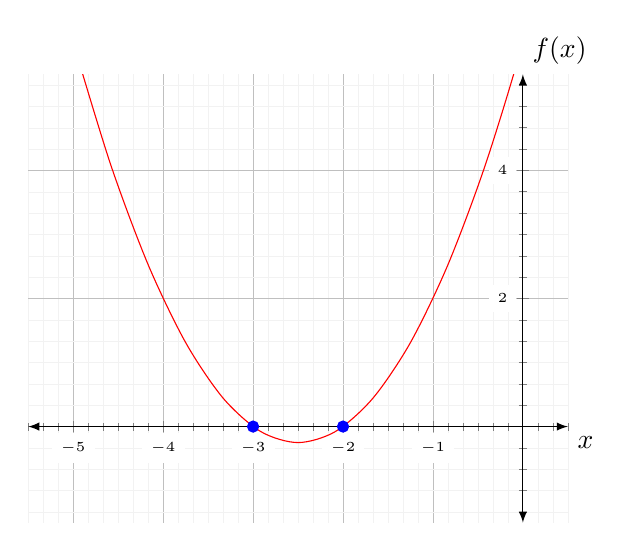
\begin{tikzpicture}
  \begin{axis}[
    xmin=-5,xmax=0,
    ymin=-1,ymax=5,
    grid=both,
    grid style={line width=.1pt, draw=gray!10},
    major grid style={line width=.2pt,draw=gray!50},
    axis lines=middle,
    minor tick num=5,
    enlargelimits={abs=0.5},
    axis line style={latex-latex},
    ticklabel style={font=\tiny,fill=white},
    xlabel style={at={(ticklabel* cs:1)},anchor=north west},
    ylabel style={at={(ticklabel* cs:1)},anchor=south west},
    xlabel=$x$,
    ylabel=$f(x)$
] 
    \addplot[smooth, red] {x^2 + 5*x +6}; 
    \addplot[only marks, blue]
        coordinates
        {(-3, 0) (-2, 0)};
  \end{axis}
\end{tikzpicture}
\end{center}

\begin{enumerate}

However, suppose that we didn't know how to factorize and want an iterative algorithm to estimate these roots.
Suppose that we start off with a point $x_0$ that just happens to be the right of $x=-2$. 



